\documentclass[conference]{IEEEtran}
\IEEEoverridecommandlockouts
% The preceding line is only needed to identify funding in the first footnote. If that is unneeded, please comment it out.
\usepackage{cite}
\usepackage{amsmath,amssymb,amsfonts}
\usepackage{algorithmic}
\usepackage{graphicx}
\usepackage{textcomp}
\usepackage{xcolor}
\def\BibTeX{{\rm B\kern-.05em{\sc i\kern-.025em b}\kern-.08em
		T\kern-.1667em\lower.7ex\hbox{E}\kern-.125emX}}

\begin{document}
	
	\title{Report Title}
	
	\makeatletter
	\newcommand{\linebreakand}{%
	\end{@IEEEauthorhalign}
	\hfill\mbox{}\par
	\mbox{}\hfill\begin{@IEEEauthorhalign}
	}
	\makeatother
	
	\author{\IEEEauthorblockN{1\textsuperscript{st} SHALOMI FERNANDES}
		\IEEEauthorblockA{\textit{Faculty of Engineering } \\
			\textit
			Bristol, UK \\
			email address or ORCID}
		\and
		\IEEEauthorblockN{2\textsuperscript{nd} FANGNAN WEI}
		\IEEEauthorblockA{\textit{Faculty of Engineering } \\
			\textit
			Bristol, UK \\
			email address or ORCID}
		\linebreakand %
		\IEEEauthorblockN{3\textsuperscript{rd} JIADONG XU}
		\IEEEauthorblockA{\textit{Faculty of Engineering } \\
			\textit
			Bristol, UK \\
			email address or ORCID}
		\and
		\IEEEauthorblockN{4\textsuperscript{th} JIAHUI LIU}
		\IEEEauthorblockA{\textit{Faculty of Engineering } \\
			\textit
			Bristol, UK \\
			ye23356@bristol.ac.uk}
	}
	
	\maketitle
	
	\begin{abstract}
		This document is a model and instructions for \LaTeX.
		This and the IEEEtran.cls file define the components of your paper [title, text, heads, etc.]. *CRITICAL: Do Not Use Symbols, Special Characters, Footnotes, 
		or Math in Paper Title or Abstract.
	\end{abstract}
	
	\section{Introduction}
	{\color{blue}A brief discussion of the problem context, motivation, analysis questions/aims and proposed methods and approaches used.}
	
	This article aims to employ machine learning to predict T-cell receptor (TCR) specificity. TCRs are critical in the immune system's ability to recognize and eliminate pathogen-infected or cancer-transformed cells. This project focuses on analyzing the vast diversity of TCR sequences from the VDJdb database, understanding how TCRs bind to specific epitopes.
	
	Predicting TCR specificity is pivotal for advancing immunotherapies and designing targeted treatments. The project involves preprocessing TCR sequence data, applying dimensionality reduction, clustering techniques, and developing algorithms to predict antigen specificity. This research holds significant potential for enhancing personalized medicine and the efficacy of immunotherapies, addressing the limitations of current empirical methods with innovative computational approaches.
	
	
	\section{Literature Review}
	{\color{blue}An overview of related work of similar research in the domain.}
	
	The IEEEtran class file is used to format your paper and style the text. All margins, 
	column widths, line spaces, and text fonts are prescribed; please do not 
	alter them. You may note peculiarities. For example, the head margin
	measures proportionately more than is customary. This measurement 
	and others are deliberate, using specifications that anticipate your paper 
	as one part of the entire proceedings, and not as an independent document. 
	Please do not revise any of the current designations.
	
	\section{Methodology}
	{\color{blue}Includes a discussion of methods applied to address your questions/aims.}
	
	Before you begin to format your paper, first write and save the content as a 
	separate text file. Complete all content and organizational editing before 
	formatting. Please note sections \ref{AA}--\ref{SCM} below for more information on 
	proofreading, spelling and grammar.
	
	Keep your text and graphic files separate until after the text has been 
	formatted and styled. Do not number text heads---{\LaTeX} will do that 
	for you.
	
	\subsection{One-Hot Encoding}\label{AA}
	One-hot encoding is a technique for representing categorical variables as binary vectors. In this encoding, the value of each variable is represented as a vector of length equal to the number of possible values, with only one element being 1 (representing the category to which the variable belongs) and all other elements being 0.
	
	Mathematical Description:
	
	Let \( X \) be a categorical variable with a finite set \( C \) of \( N \) categories, such that:
	\[ X \in C = \{ c_1, c_2, \ldots, c_N \} \]
	
	Here, each \( c_i \) represents a distinct category.
	
	Corresponding to each category \( c_i \) of \( X \), we define a one-hot vector \( d_i \) as a binary vector of length \( N \). This vector has all elements set to 0 except for the \( i \)-th element, which is set to 1.

	For a given category \( c_i \), its one-hot vector \( d_i \) is given by:
	\[ d_i = (0, 0, \ldots, 1, \ldots, 0) \]
	
	Here, the 1 is in the \( i \)-th position of the vector \( d_i \), indicating the presence of category \( c_i \).
	
	We can also define one-hot encoding using an indicator function \( I \) as follows:
	\[ d_{i}[j] = I(j = i) \]
	
	Where:
	\[ I(true) = 1 \quad \text{and} \quad I(false) = 0 \]
	
	The indicator function \( I \) returns 1 when its argument is true (when \( j = i \)), and 0 otherwise.
	
	The one-hot vector \( d_i \) can be represented as:
	\[ d_i = [d_{i}[1], d_{i}[2], \ldots, d_{i}[N]] \]
	
	Where:
	\[ d_{i}[j] = 
	\begin{cases} 
		1 & \text{if } j = i \\ 
		0 & \text{if } j \neq i 
	\end{cases}
	\]
	
	First, we specify that the parameters of the function are cdr3\_sequence and an optional sequence max\_length to specify the maximum length of the encoded sequence, and to iterate over each amino acid in the cdr3\_sequence with its corresponding one-hot encoding set to 1 and the rest of the positions set to 0. If the length of the cdr3\_sequence is less than max\_length, a zero vector is padded at the end of the encoded sequence, and if the length of the cdr3\_sequence is greater than max\_length, the first max\_length lines of the encoded sequence are truncated.

	\subsection{Biological Encoding}\label{AA}
	
	Biocoding refers to the process of converting biological entities (such as proteins, DNA, RNA, etc.) into a form that can be processed by a computer. In this paper, BLOSUM90 is used as a biological code, BLOSUM90 a type of protein sequence coding. In the BLOSUM90, each amino acid is converted to a vector, and each element of the vector represents an amino acid's similarity score with other amino acids. This similarity score is usually derived from the BLOSUM matrix, which contains information about the frequency of substitution between different amino acids. In the coding, '-' represents the missing amino acid and is usually given a minimum or median to indicate its difference from other amino acids.
	
	We first created biological matrix loading functions (e.g., BLOSUM90(), BLOSUM62()) that are used to load protein sequence alignment score matrices commonly used in bioinformatics, in which only the amino acids in the standard protein letter sequences are retained, and the rest are filled with specific values.
	
	For each amino acid in the input CDR3 sequence, a biological matrix is used to convert it to a vector representation, with a zero vector at the end of the encoded sequence if the length of the cdr3\_sequence is less than max\_length, and the first max\_length elements of the encoded sequence truncated if the length of the cdr3\_sequence is greater than max\_length.
	
	\subsection{Levenshtein}\label{AA}
	A method used to measure the similarity between two strings, which represents the minimum number of editing operations required to convert one string to another.
	
	\subsection{GIANA}\label{AA}
	GIANA is a tool for analyzing immune cell receptor sequence data, which calculates the distance between sequences and similarity matrices. By passing the data of the alpha chain and the beta chain to the GIANA script separately, and specifying the output directory, the corresponding distance and similarity matrix files can be generated.
	
	\subsection{TCRDist}\label{AA}
	TCRDist is a toolkit for calculating TCR distances, which can be calculated based on their sequence characteristics (e.g., CDR3 sequences) and possibly other information (e.g., expression patterns of TCRs).
	
	For a given set of TCR sequences, the distances between all possible pairs are calculated, and the results are formed into a distance matrix, each element in the matrix represents the distance or similarity between the pairs, and once the distance matrix is calculated, visualization tools can be used to show the similarity or difference between the TCRs.
	
	\subsection{PCA}\label{AA}
	PCA (Principal Component Analysis) is used to project a high-dimensional dataset into a low-dimensional space, by finding the principal variance directions (principal components) in the data, and then projecting the data onto these directions, so as to achieve dimensionality reduction of the data.
	
	Given a dataset \( X \) with \( n \) samples and \( d \) features, where \( X \) is an \( n \times d \) matrix, PCA aims to find a \( k \)-dimensional linear subspace that maximally preserves the variance of the original data. This subspace is defined by the \( k \) most important principal components.
	
	\text{Compute the mean vector of the data: } 
	$\bar{x} = \frac{1}{n} \sum_{i=1}^{n} x_i$
	
	Standardize the data: Subtract the mean vector from each sample to obtain the centered data: \( \tilde{X} = X - \bar{x} \)
	
	Compute the covariance matrix of the data: \( \Sigma = \frac{1}{n} \tilde{X}^T \tilde{X} \)
	
	Perform the eigendecomposition of the covariance matrix: $\Sigma = V \Lambda V^T$, where $V$ is the matrix containing the eigenvectors and $\Lambda$ is a diagonal matrix containing the eigenvalues.
	
	Select the top \(k\) eigenvectors corresponding to the largest eigenvalues: \(V_k = \begin{bmatrix} | & | & & | \\ v_1 & v_2 & \cdots & v_k \\ | & | & & | \end{bmatrix}\)
	
	Project the original data onto the selected principal components: \(Z = \tilde{X} V_k\)
	
	Through these steps, we obtain a lower-dimensional dataset \(Z\) with dimensions \(n \times k\). In this subspace, the variance of the data is maximally preserved, and the principal components \(v_i\) represent the most important directions in the data.
	\subsection{t-SNE}\label{AA}
	t-SNE is a nonlinear dimensionality reduction algorithm designed to map high-dimensional data to two- or three-dimensional space. t-SNE first calculates the similarity between data points in the high-dimensional space, and then maintains this similarity relationship in the low-dimensional space, using the t-distribution to represent the distance between the data points in the low-dimensional space, which helps to preserve the local structure of the data.
	
	\subsection{UMAP}\label{AA}
	UMAP (\emph{Uniform Manifold Approximation and Projection}) is a nonlinear dimensionality reduction algorithm, similar to t-SNE, but with faster computation speed and better ability to maintain the global structure than t-SNE.
	
	UMAP achieves dimensionality reduction and visualization through the following steps: first, calculate the similarity between data points, and then construct a neighborhood map to represent the local relationship between data points, second, optimize the manifold structure in the high-dimensional space to keep the distance of adjacent data points in the low-dimensional space as similar as possible, and finally, map the optimized manifold structure to the low-dimensional space to generate a new low-dimensional representation for visualization and analysis.
	\subsection{DecisionTreeClassifier}\label{AA}
	DecisionTreeClassifier is a tree-based supervised learning algorithm for classifying and regressing data. In the classification task, the decision tree generates a tree by performing a series of splits on the input features, with each split node representing a feature and each leaf node representing a category.
	\begin{itemize}
		\item Feature Selection: Select the best split feature from the input features so that the split on that feature maximizes the purity of the data.
		\item Split nodes: Split the data based on the selected features to generate sub-nodes so that each sub-node contains samples that belong to the same category as much as possible.
		\item Recursive build: Repeat the above process for each child node until the stop condition is met.
		\item Prediction: The test sample is traversed along the branches of the tree to the leaf node, and the category of the leaf node is used as the prediction.
	\end{itemize}
	
	In this paper, the dataset is divided into training sets and datasets, where 70\% of the data is used for training and 30\% for testing, the same random seed random\_state=42 is used for each experiment, the accuracy of each experiment is recorded, and the average accuracy of 20 experiments is calculated.
	
	\subsection{RnadomForestClassifier}\label{AA}
	RandomForestClassifier is an ensemble learning method that consists of multiple decision trees, each trained on a different random subset, and ultimately averages their predictions. Compared with a single decision tree, random forests generally provide better generalization performance and are more robust to high-dimensional data and noise in the data.
	
	In this paper, the dataset is divided into a training set and a dataset, with 70\% of the data used for training and 30\% for testing, stratified sampling of the target variable (epitope) to keep the proportion of each category in the training set and test set up the same as in the original dataset, and RandomForestClassifier is used to build a model with 80 trees.
	
	\subsection{Agglomerative Hierarchical Clustering}\label{AA}
	Agglomerative Hierarchical Clustering is a clustering algorithm that gradually merges data points into clusters, and represents the similarity relationship between data points through a tree-like structure. Agglomerative Hierarchical Clustering takes the distance between data points as a measure of similarity, and then gradually merges the data points into different clusters based on preset parameters (number of clusters, distance metric, and linking method).
	
	Mathematical Description:
	
	Start by treating each data point as a single cluster. Let $C = \{C_1, C_2, \ldots, C_N\}$ be the initial set of clusters where each $C_i$ contains a single data point. Define a similarity measure (or distance measure) $d(C_i, C_j)$ between two clusters $C_i$ and $C_j$.
	
	Find the closest (most similar) pair of clusters and merge them into a single cluster.Mathematically, if $C_i$ and $C_j$ are the closest pair, they are merged to form a new cluster $C_k$.
	
	After merging $C_i$ and $C_j$, update the distance matrix to reflect the distances of the new cluster $C_k$ to all existing clusters. 
	\begin{itemize}
		\item \textbf{Single Linkage}:
		
		 $d(C_k, C_x) = \min(d(C_i, C_x), d(C_j, C_x))$
		\item \textbf{Complete Linkage}: 
		
		$d(C_k, C_x) = \max(d(C_i, C_x), d(C_j, C_x))$
		\item \textbf{Average Linkage}: 
		
		$d(C_k, C_x) = \frac{d(C_i, C_x) + d(C_j, C_x)}{2}$
		\item \textbf{Ward's Method}: Merge the pair of clusters that results in the minimum increase in total within-cluster variance after merging.
	\end{itemize}
	
	Repeat these steps until all data points are clustered into a single cluster of size $N$. As clusters are merged, a tree-like diagram called a dendrogram is created to record the sequences of merges. This dendrogram illustrates how each cluster is composed by branching out to its constituent elements.
	
	In this paper, the number of clusters was set to 5, and the similarity between the clustering results and the real labels and the clustering quality were evaluated by using the Adjusted Rand Index and Silhouette Score. The Adjusted Rand Index measures how similar the clustering results are to the real labels, with values between -1 and 1, with closer to 1 indicating that the clustering results are more similar to the real labels. The Silhouette Score measures the clustering closeness of each sample and ranges from -1 to 1, with closer to 1 indicating better clustering results.
	
	\subsection{DBSCAN}\label{AA}
	DBSCAN is a popular clustering algorithm that identifies clusters of different shapes and sizes in a dataset, unlike methods such as K-means, DBSCAN does not require pre-specifying the number of clusters to be identified.
	
	For each point in the dataset, DBSCAN calculates how many points are within that eps (the maximum distance between two points, where one point is considered to be within the neighborhood of the other point, and the smaller the value, the more clustering) distance. If the count exceeds min\_samples (the minimum number of points required to form a dense area, higher values usually result in more points being treated as noise), then the point is marked as a core point; Starting from a core point, DBSCAN recursively finds all the points that are dense from that point and assigns them to the same cluster; Neither the core nor any core point where the direct density is reachable is marked as noise.
	
	\subsection{Some Common Mistakes}\label{SCM}
	\begin{itemize}
		\item The word ``data'' is plural, not singular.
		\item Do not use the word ``essentially'' to mean ``approximately'' or ``effectively''.
		\item In your paper title, if the words ``that uses'' can accurately replace the word ``using'', capitalize the ``u''; if not, keep using lower-cased.
		\item Be aware of the different meanings of the homophones ``affect'' and ``effect'', ``complement'' and ``compliment'', ``discreet'' and ``discrete'', ``principal'' and ``principle''.
		\item Do not confuse ``imply'' and ``infer''.
		\item The prefix ``non'' is not a word; it should be joined to the word it modifies, usually without a hyphen.
		\item There is no period after the ``et'' in the Latin abbreviation ``et al.''.
		\item The abbreviation ``i.e.'' means ``that is'', and the abbreviation ``e.g.'' means ``for example''.
	\end{itemize}
	An excellent style manual for science writers is \cite{b7}.
	
	
	\subsection{Figures and Tables}
	\paragraph{Positioning Figures and Tables} Place figures and tables at the top and 
	bottom of columns. Avoid placing them in the middle of columns. Large 
	figures and tables may span across both columns. Figure captions should be 
	below the figures; table heads should appear above the tables. Insert 
	figures and tables after they are cited in the text. Use the abbreviation 
	``Fig.~\ref{fig}'', even at the beginning of a sentence.
	
	\begin{table}[htbp]
		\caption{Table Type Styles}
		\begin{center}
			\begin{tabular}{|c|c|c|c|}
				\hline
				\textbf{Table}&\multicolumn{3}{|c|}{\textbf{Table Column Head}} \\
				\cline{2-4} 
				\textbf{Head} & \textbf{\textit{Table column subhead}}& \textbf{\textit{Subhead}}& \textbf{\textit{Subhead}} \\
				\hline
				copy& More table copy$^{\mathrm{a}}$& &  \\
				\hline
				\multicolumn{4}{l}{$^{\mathrm{a}}$Sample of a Table footnote.}
			\end{tabular}
			\label{tab1}
		\end{center}
	\end{table}
	
	\begin{figure}[htbp]
%		\centerline{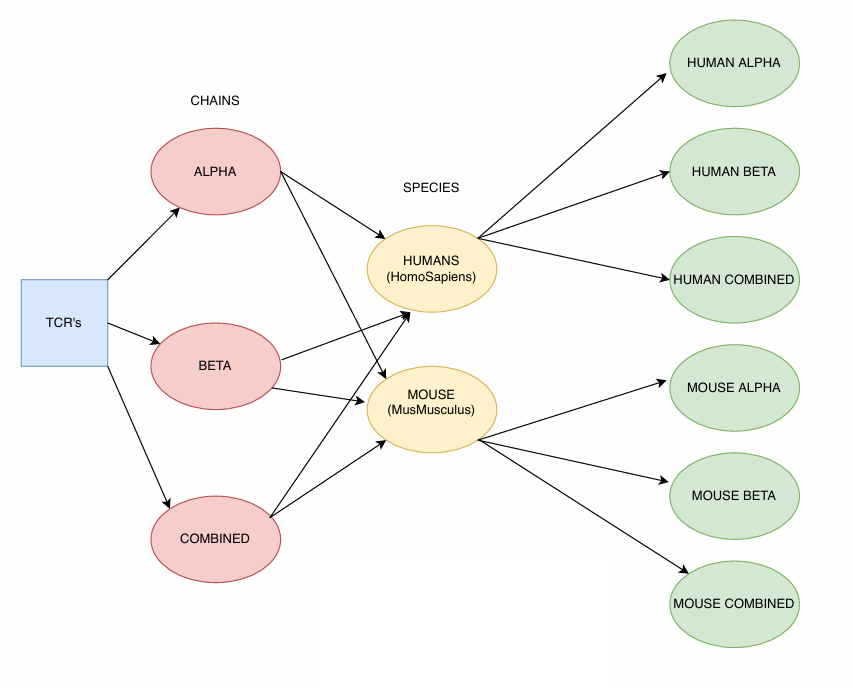
\includegraphics{fig1.png}}
		\caption{Example of a figure caption.}
		\label{fig}
	\end{figure}
	
	Figure Labels: Use 8 point Times New Roman for Figure labels. Use words 
	rather than symbols or abbreviations when writing Figure axis labels to 
	avoid confusing the reader. As an example, write the quantity 
	``Magnetization'', or ``Magnetization, M'', not just ``M''. If including 
	units in the label, present them within parentheses. Do not label axes only 
	with units. In the example, write ``Magnetization (A/m)'' or ``Magnetization 
	\{A[m(1)]\}'', not just ``A/m''. Do not label axes with a ratio of 
	quantities and units. For example, write ``Temperature (K)'', not 
	``Temperature/K''.
	
	\subsection{References}
	
	Please number citations consecutively within brackets \cite{b1}. The 
	sentence punctuation follows the bracket \cite{b2}. Refer simply to the reference 
	number, as in \cite{b3}---do not use ``Ref. \cite{b3}'' or ``reference \cite{b3}'' except at 
	the beginning of a sentence: ``Reference \cite{b3} was the first $\ldots$''
	
	Capitalize only the first word in a paper title, except for proper nouns and 
	element symbols.
	
	\section{Data Description / Preparation}
	{\color{blue}Includes description of data sources, samples and steps for pre-processing if any.}
	\subsection{Data Processing}
	\begin{itemize}
		\item Data filtering: Select specific columns ('complex.id', 'gene', 'cdr3', 'v.segm', 'j.segm', 'species', 'mhc.a', 'mhc.b', 'mhc.class', 'antigen.epitope') from the complete dataset to create a new DataFrame: filtered\_data.
		\item Missing value checking and processing: Because V and J are important factors when analyzing TCR characteristics, the rows with missing values in the columns 'v.segm' and 'j.segm' were removed from the new dataset filtered\_data.
		\item Data Segmentation and Reprocessing: In order to process the TCR sequences of alpha and beta chains separately, the data is divided into two new DataFrames based on the value of the 'gene' column: cdr3\_alpha\_df (rows containing 'gene' with 'TRA') and cdr3\_beta\_df (rows containing 'gene' with 'TRB') values. Remove the 'gene' column from the two new DataFrames, as the information in that column is already redundant after splitting the data.
		\item Data merging: cdr3\_alpha\_df and cdr3\_beta\_df were combined according to the columns 'complex.id', 'species', 'mhc.a', 'mhc.b', 'mhc.class', 'antigen.epitope'. Suffix different TCR strand feature columns, such as CDR3, V-segment, and J-segment, to distinguish datasets.
		
	\end{itemize}
	
	
	\section{Results and Discussion}
	{\color{blue}Reporting on the experiments with discussion on insights. Technical challenges are to be discussed here too.}
	
	\section{Further Work and Improvement}
	{\color{blue}Explore what can be done further based on the discussed insights and ways to improve.}
	
	\section{Conclusion}
	{\color{blue}A brief summary of the key insights in your report.}
	
	\begin{thebibliography}{00}
		\bibitem{b1} G. Eason, B. Noble, and I. N. Sneddon, ``On certain integrals of Lipschitz-Hankel type involving products of Bessel functions,'' Phil. Trans. Roy. Soc. London, vol. A247, pp. 529--551, April 1955.
		\bibitem{b2} J. Clerk Maxwell, A Treatise on Electricity and Magnetism, 3rd ed., vol. 2. Oxford: Clarendon, 1892, pp.68--73.
		\bibitem{b3} I. S. Jacobs and C. P. Bean, ``Fine particles, thin films and exchange anisotropy,'' in Magnetism, vol. III, G. T. Rado and H. Suhl, Eds. New York: Academic, 1963, pp. 271--350.
		\bibitem{b4} K. Elissa, ``Title of paper if known,'' unpublished.
		\bibitem{b5} R. Nicole, ``Title of paper with only first word capitalized,'' J. Name Stand. Abbrev., in press.
		\bibitem{b6} Y. Yorozu, M. Hirano, K. Oka, and Y. Tagawa, ``Electron spectroscopy studies on magneto-optical media and plastic substrate interface,'' IEEE Transl. J. Magn. Japan, vol. 2, pp. 740--741, August 1987 [Digests 9th Annual Conf. Magnetics Japan, p. 301, 1982].
		\bibitem{b7} M. Young, The Technical Writer's Handbook. Mill Valley, CA: University Science, 1989.
	\end{thebibliography}
	
	\appendix
	{\color{blue}The document up to this section should be no more than 8 pages. The appendix section is optional. You can include additional material here, but it will not be marked.}
	
\end{document}
